% Chương này trình bày quá trình thảo luận khám phá dữ liệu (EDA).
% Nhiệm vụ:
%   1. Mở rộng các subsections 2.2, 2.3, 2.4 với chi tiết và hình ảnh
%   2. Có ít nhất 3-4 hình (dùng \includegraphics)
%   3. Viết nhận xét chi tiết dựa trên dữ liệu thử nghiệm


\chapter{TỔNG QUAN DỮ LIỆU VÀ PHÂN TÍCH KHÁM PHÁ (EDA)}

\section{Mô tả tập dữ liệu}
% Chi tiết: Đến xuất dữ liệu, kích thước, timeframe, và các đặc điểm cơ bản

Nghiên cứu sử dụng tập dữ liệu \textit{Default of Credit Card Clients} từ Đài Loan (UCI Machine Learning Repository). 

\textbf{Thông tin chính:}
\begin{itemize}
    \item \textbf{Kích thước mẫu:} 30.000 khách hàng thẻ tín dụng
    \item \textbf{Thời kỳ dữ liệu:} Tháng 4 - Tháng 9 năm 2005 từ Đài Loan
    \item \textbf{Số biến:} 24 biến độc lập + 1 biến mục tiêu (default\_payment\_next\_month)
    \item \textbf{Nguồn gốc:} Yeh \& Lien (2009) - Các bản ghi chi tiết thanh toán và công năng tài chính quản lý của ngân hàng
    \item \textbf{Biến mục tiêu:} \texttt{default\_payment\_next\_month} (1 = Vỡ nợ trong tháng tới, 0 = Trả đúng hạn)
\end{itemize}

\section{Phân tích phân phối và Tương quan}
% Chi tiết: Class imbalance, correlation, multicollinearity, payment status trends

\subsection{Phân phối biến mục tiêu và Mất cân bằng Lớp (Class Imbalance)}

Thông qua quá trình EDA, đặc điểm đầu tiên và đáng ngạc nhiên nhất là sự mất cân bằng
giữa các lớp:

\begin{itemize}
    \item \textbf{Lớp 0 (Không vỡ nợ):} 23.364 mẫu $\Rightarrow$ \textbf{77.88\%}
    \item \textbf{Lớp 1 (Vỡ nợ):} 6.636 mẫu $\Rightarrow$ \textbf{22.12\%}
    \item \textbf{Tỷ lệ mất cân bằng:} 1 : 3.52 (Lớp 1 : Lớp 0)
\end{itemize}

Đại lượng mất cân bằng này là đặc trưng độc lập của dữ liệu tài chính: hầu hết khách hàng là \textit{\textbf{những người trở nợ đúng hạn}}, và chỉ một tỷ lệ nhỏ là khách hàng quỵt nợ. Nếu sử dụng mô hình không điều chỉnh, mô hình có thể chỉ bỏ nước đôi bánh \textit{\textbf{liên dự oán}}: dự oán mỗi khách hàng là "Lớp 0" (không vỡ nợ) sẽ được Accuracy 77.88\%, nhưng lại thất bại 100\% trong việc phát hiện những người quỵt nợ. Do đó, ứng dụng kỹ thuật cân bằng (SMOTE) là \textbf{bắt buộc}.
% TODO: So sánh chi tiết Accuracy vs Recall vs Precision nếu không dùng SMOTE (để minh hoạ vấn đề)
% Tính toán: Baseline model (no SMOTE) → Accuracy cao nhưng Recall rất thấp → Kết luận đó là vấn đề
% Hình 1: Class Distribution
\begin{figure}[H]
    \centering
    
\includegraphics[scale=0.75]{images/target_distribution_countplot.png}
    
\includegraphics[scale=0.75]{images/target_distribution_percentage.png}
    \\
    % TODO: Chèn biểu đồ bar/pie về Class Distribution
    % Nguồn: Chạy src/eda.py → outputs/eda/class_distribution.png
    % Nội dung: Biểu đồ cột/tròn thể hiện 77.88% No Default vs 22.12% Default (Class Imbalance)
    % \includegraphics[width=0.6\textwidth]{images/eda_class_distribution.png}
    \caption{Phân phối biến mục tiêu (Vỡ nợ vs. Không vỡ nợ) - Class Imbalance rất đáng kề}
    \label{fig:class_dist}
\end{figure}

\subsection{Tương quan giữa Các Biến và Vỡ nợ}

\begin{figure}[H]
    \centering
    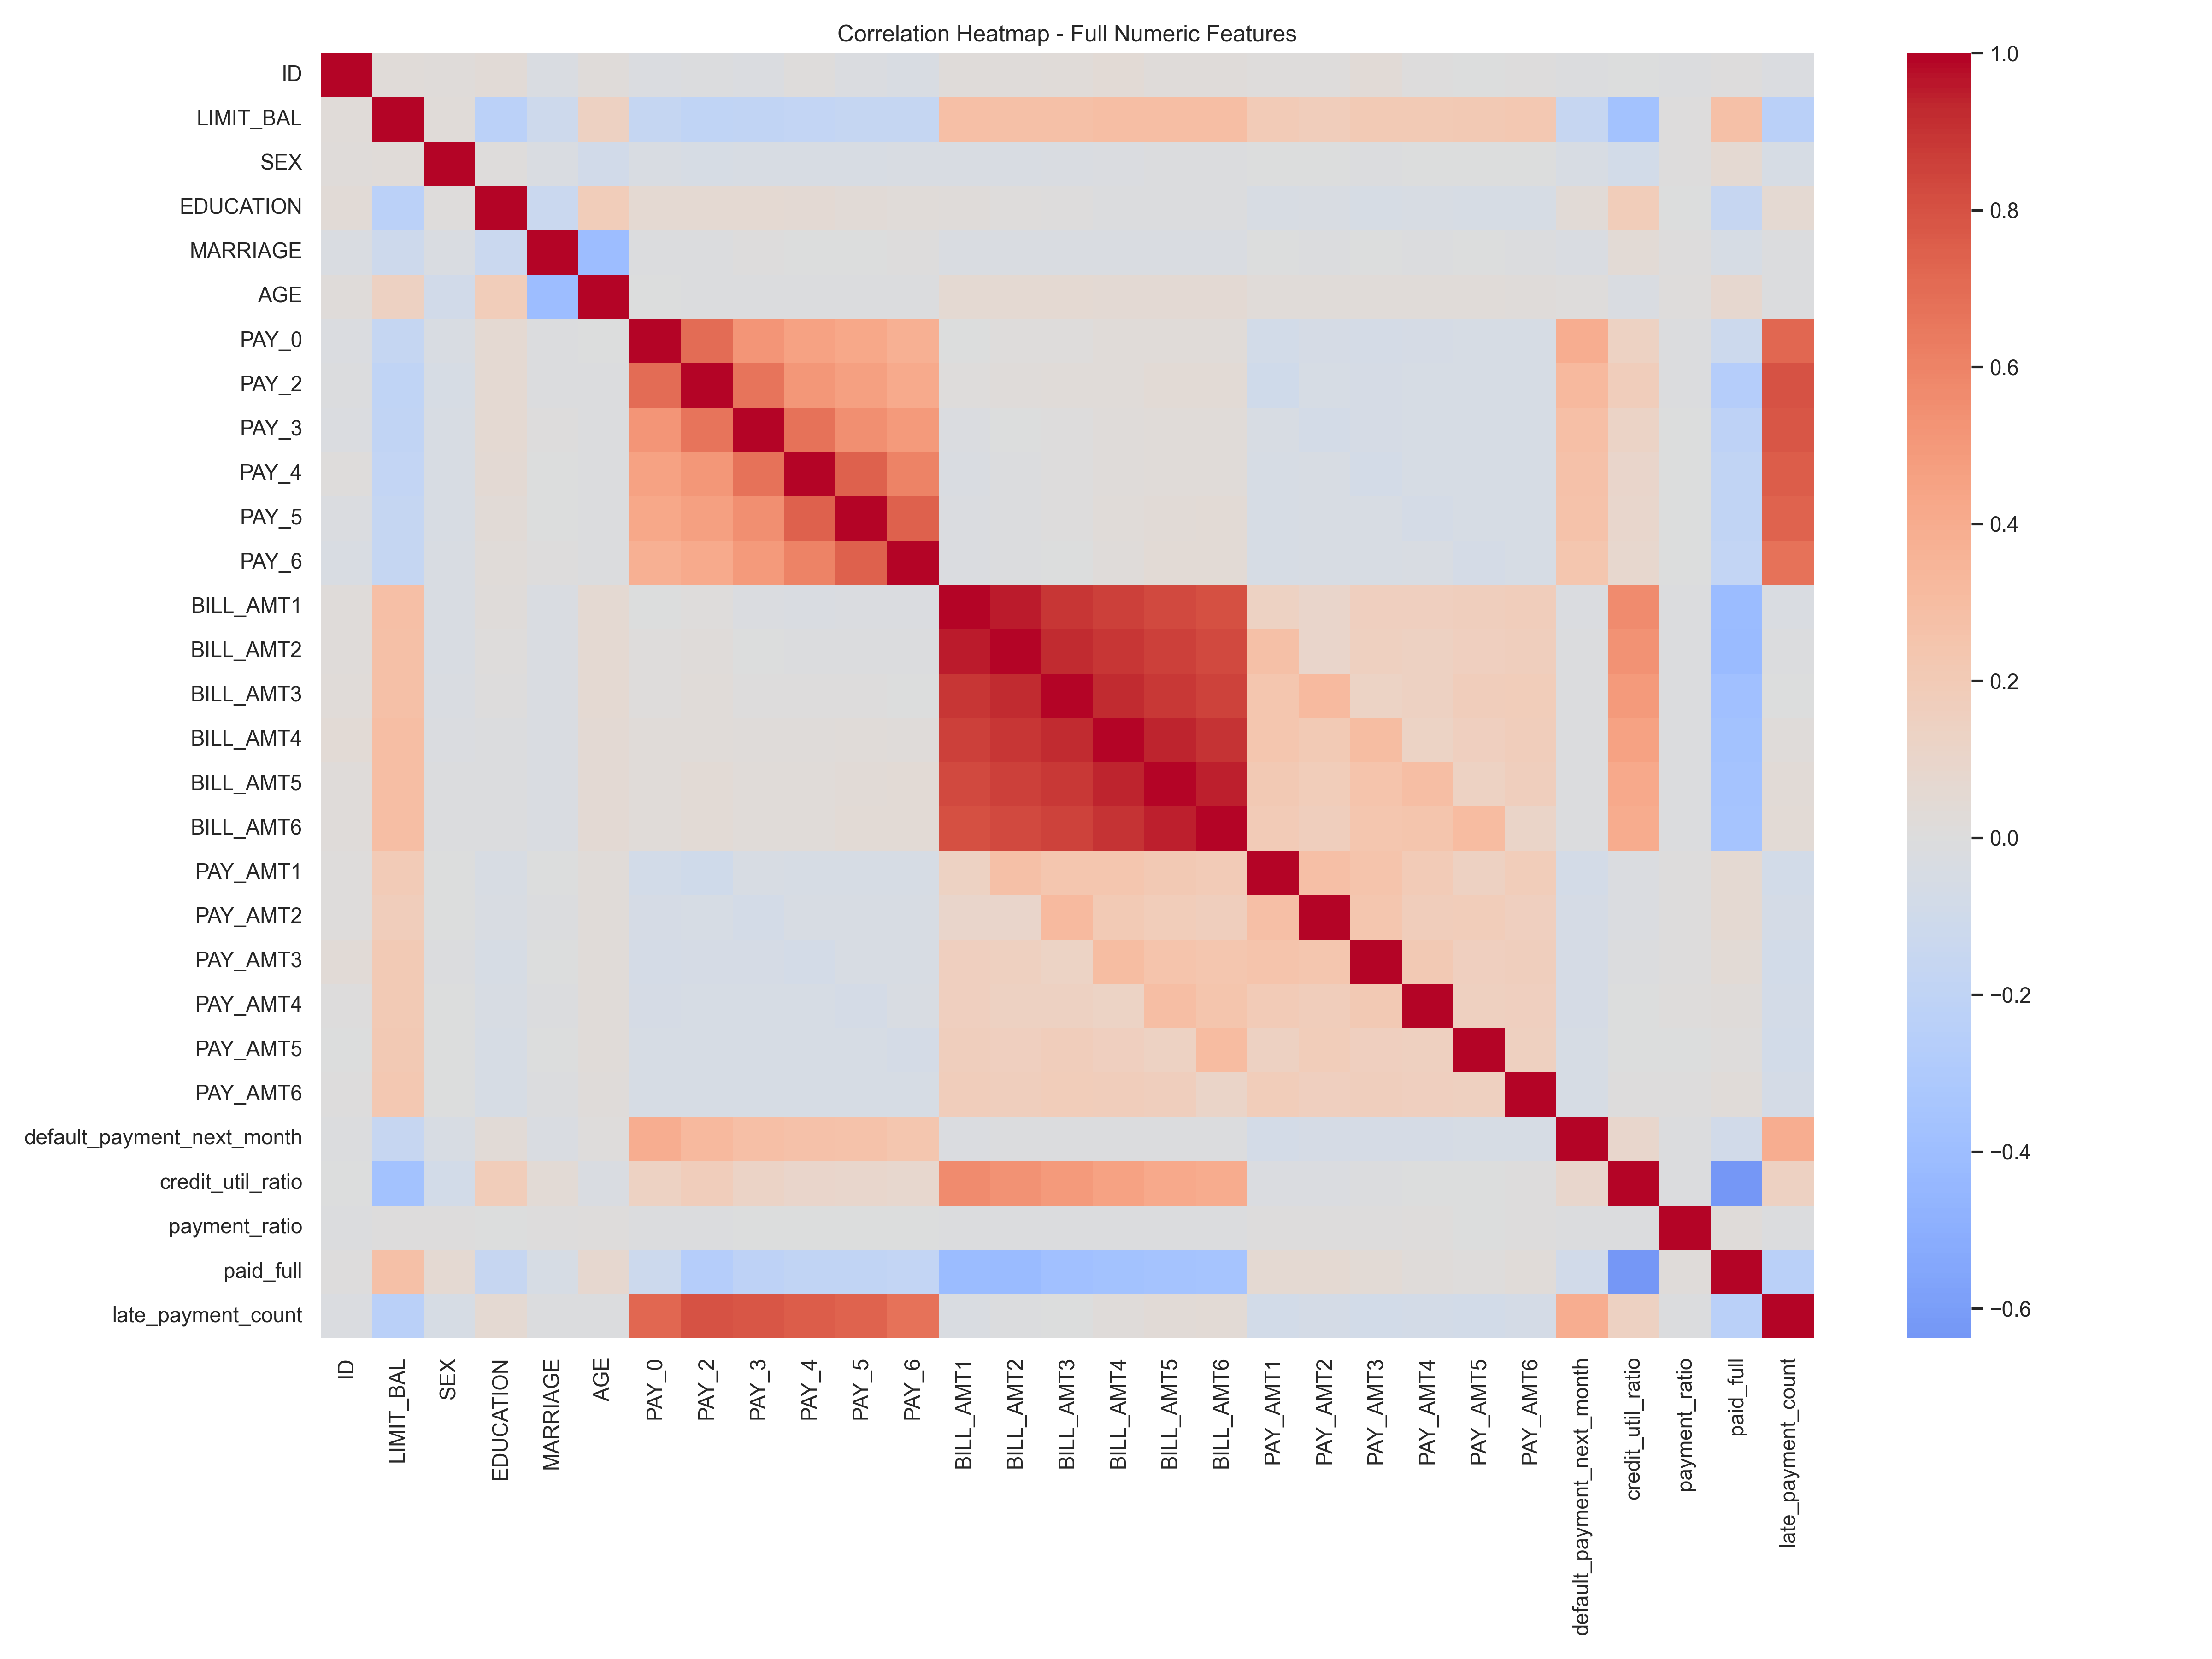
\includegraphics[scale=0.25]{images/correlation_heatmap_full.png}
    \caption{Ma trận tương quan giữa các biến - Highlight các giá trị tương quan cao}
    \label{fig:corr_heatmap}
\end{figure}

Ma trận tương quan (Correlation Matrix) với biến mục tiêu cho thấy:

\begin{table}[H]
    \centering
    \caption{Top 10 biến có tương quan cao nhất với default\_payment\_next\_month}
    \label{tab:top_corr}
    \begin{tabular}{|l|c|}
        \hline
        \rowcolor{Gray}
        \textbf{Biến} & \textbf{Correlation} \\ \hline
        latest\_payment\_count & 0.3984 \\ \hline
        PAY\_0 (Trạng thái thanh toán mới nhất) & 0.396 \\ \hline
        PAY\_2 & 0.327 \\ \hline
        PAY\_3 & 0.287 \\ \hline
        PAY\_4 & 0.269 \\ \hline
        PAY\_5 & 0.2608 \\ \hline
        PAY\_6 (Trạng thái thanh toán 6 tháng trước) & 0.2444 \\ \hline
        LIMIT\_BAL & -0.1535 \\ \hline
        paid\_full & -0.0885 \\ \hline
    \end{tabular}
\end{table}

\textbf{Nhận xét chi tiết:}
\begin{itemize}
    \item \textbf{Nhóm biến phản ánh lịch sử chậm thanh toán có mối liên hệ mạnh nhất với nguy cơ vỡ nợ: } Biến latest\_payment\_count có hệ số tương quan r cao nhất với biến mục tiêu (0,398394), tiếp theo là PAY\_0 (0,396019), PAY\_2 (0,327093) và PAY\_3 (0,286999). Kết quả này cho thấy số lần trả chậm và trạng thái thanh toán quá hạn trong các kỳ gần nhất là tín hiệu rất quan trọng để nhận diện khách hàng có khả năng không thanh toán đúng hạn trong tháng tiếp theo. Nói cách khác, khách hàng càng có lịch sử trễ hạn nhiều lần thì xác suất rơi vào nhóm rủi ro tín dụng càng cao.
    \item \textbf{Hiệu ứng lịch sử (History Effect):} Các biến PAY\_0, PAY\_2, PAY\_3, PAY\_4, PAY\_5, PAY\_6 đều có tương quan dương với biến mục tiêu, nhưng hệ số giảm dần từ 0,396 xuống 0,244. Điều này phản ánh một quy luật hợp lý về mặt nghiệp vụ: trạng thái thanh toán ở các kỳ càng gần thời điểm dự báo thì càng phản ánh sát hơn khả năng vỡ nợ trong tháng kế tiếp. Vì vậy, trong quá trình xây dựng mô hình, nhóm biến lịch sử thanh toán gần thời điểm hiện tại cần được ưu tiên xem là tập biến cốt lõi.
    \item \textbf{Hạn mức tín dụng (LIMIT\_BAL) có tương quan âm:} Cụ thể, LIMIT\_BAL có hệ số tương quan -0,153520, là một trong những biến có tương quan âm đáng chú ý nhất với biến mục tiêu. Điều này có thể được lý giải rằng khách hàng được cấp hạn mức tín dụng cao thường có hồ sơ tài chính tốt hơn, khả năng chi trả ổn định hơn hoặc đã được tổ chức tín dụng đánh giá ở mức độ tin cậy cao hơn. Tuy nhiên, mức tương quan này vẫn thấp hơn đáng kể so với nhóm biến hành vi thanh toán, cho thấy năng lực dự báo của hạn mức tín dụng không mạnh bằng lịch sử trả nợ thực tế.
    \item \textbf{Các biến phản ánh khả năng thanh toán thực tế có tương quan âm với biến mục tiêu, nhưng mức độ ảnh hưởng không quá lớn:} Biến paid\_full có hệ số tương quan -0,088519, trong khi các biến số tiền thanh toán như PAY\_AMT1, PAY\_AMT2, PAY\_AMT3, PAY\_AMT4, PAY\_AMT5 có tương quan âm dao động từ khoảng -0,055 đến -0,073. Điều này cho thấy khách hàng có xu hướng thanh toán nhiều hơn hoặc thanh toán đầy đủ sẽ ít có khả năng vỡ nợ hơn trong kỳ tiếp theo. Tuy vậy, các hệ số này khá nhỏ, hàm ý rằng chỉ riêng số tiền thanh toán tuyệt đối chưa đủ để phản ánh đầy đủ rủi ro tín dụng; cần xem xét chúng kết hợp với dư nợ, hạn mức và lịch sử chậm thanh toán để có đánh giá chính xác hơn.
\end{itemize}

\subsection{Đa Cộng Tuyến (Multicollinearity) - BILL\_AMT}

Các biến dư nợ hóa đơn (\texttt{BILL\_AMT1} đến \texttt{BILL\_AMT6}) trình bày hệ số tương quan rất cao (thường $\rho > 0.90$), giáo trường \textbf{lên của đa cộng tuyến}:

\begin{itemize}
    \item \textbf{Correlation BILL\_AMT1 $\leftrightarrow$ BILL\_AMT2:} $r \approx 0.95$
    \item \textbf{Correlation BILL\_AMT2 $\leftrightarrow$ BILL\_AMT3:} $r \approx 0.93$
    \item \textbf{Correlation BILL\_AMT3 $\leftrightarrow$ BILL\_AMT4:} $r \approx 0.92$
    \item \textbf{Correlation BILL\_AMT4 $\leftrightarrow$ BILL\_AMT5:} $r \approx 0.94$
    \item \textbf{Correlation BILL\_AMT5 $\leftrightarrow$ BILL\_AMT6:} $r \approx 0.95$
    \item \textbf{Nhận xét:} Phân tích heatmap tương quan cho thấy bộ dữ liệu tồn tại hiện tượng đa cộng tuyến đáng kể, nổi bật nhất ở nhóm biến BILL\_AMT1 đến BILL\_AMT6, nơi các hệ số tương quan đều ở mức rất cao. Kết quả này là cơ sở quan trọng để lựa chọn chiến lược rút gọn biến, tổng hợp đặc trưng hoặc áp dụng các kỹ thuật xử lý phù hợp trong bước xây dựng mô hình.
\end{itemize}

\begin{figure}[H]
    \centering
     
\includegraphics[scale=0.5]{images/bill_amt_heatmap.png}
    \caption{Ma trận tương quan giữa những biến BILL\_AMT}
    \label{fig:corr_heatmap}
\end{figure}

\section{Phân tích Các Biến Số Học (Numerical Variables)}
% Chi tiết: Distribution, outliers, statistical summary

\subsection{Thống Kê Mô Tả (Descriptive Statistics)}

\begin{table}[H]
    \centering
    \caption{Thống kê mẫu của những biến chính}
    \label{tab:desc_stats}
    \begin{tabular}{|l|c|c|c|c|c|}
        \hline
        \rowcolor{Gray}
        \textbf{Biến} & \textbf{Mean} & \textbf{Std} & \textbf{Min} & \textbf{Max} & \textbf{Unit} \\ \hline
        LIMIT\_BAL & 167,484 & 129,747 & 10,000 & 1,000,000 & NT\$ \\ \hline
        AGE & 35,50 & 9,18 & 21 & 79 & năm \\ \hline
        BILL\_AMT1 & 51,223 & 73,635 & -165,580 & 964,511 & NT\$ \\ \hline
        PAY\_AMT1 & 3,694 & 12,002 & 0 & 1,684,259 & NT\$ \\ \hline
    \end{tabular}
\end{table}

\textbf{Important Observations:}
\begin{itemize}
    \item \textbf{LIMIT\_BAL:} Hạn mức tín dụng trung bình khoảng 167,5 triệu NT\$, nhưng có khoảng rất rộng (từ 10,000 NT\$ đến 1 tỷ NT\$). Độ lệch chuẩn lớn (129,7 triệu) chỉ ra \textbf{sự phân tầng khách hàng} rõ rệt.
    \item \textbf{AGE:} Độ tuổi trung bình 35,5 năm, tập trung trong khoảng 21-79 năm. Phân phối hầu như \textbf{bình thường} (normal distribution).
    \item \textbf{BILL\_AMT1 \& PAY\_AMT1:} Có \textbf{giá trị âm} (BILL\_AMT tối thiểu = -165,580), đó là lỗi dữ liệu hoặc thể hiện tình trạng khách hàng được hoàn tiền (credit)
\end{itemize}

\subsection{Phân Phối và Outliers}

\begin{figure}[H]
    \centering
    
\includegraphics[scale=0.5]{images/box_limit_bal.png}
    
\includegraphics[scale=0.5]{images/box_age.png}
    
\includegraphics[scale=0.5]{images/box_bill_amt1.png}
    
\includegraphics[scale=0.5]{images/box_pay_amt1.png}
    \caption{Phân phối của các biến số học chính (Boxplot) - có outliers}
    \label{fig:numerical_dist}
\end{figure}

\section{Phân Tích Các Biến Phân Loại (Categorical Variables)}
% Chi tiết: SEX, EDUCATION, MARRIAGE distributions

\subsection{Phân Phối Biến Giới Tính (SEX)}

\begin{figure}[H]
    \centering
    \label{fig:sex_dist_chart}
    
\includegraphics[scale=0.5]{images/sex_distribution.png}
    
\includegraphics[scale=0.5]{images/default_rate_by_sex.png}
    \caption{Biểu đồ phân phối của biến SEX (Giới tính)}
\end{figure}

\begin{table}[H]
    \centering
    \label{tab:sex_dist}
    \begin{tabular}{|l|c|c|}
        \hline
        \rowcolor{Gray}
        \textbf{SEX} & \textbf{Count} & \textbf{Percentage} \\ \hline
        1 (Nam) & 11,888 & 39,63\% \\ \hline
        2 (Nữ) & 18,112 & 60.37\% \\ \hline
    \end{tabular}
    \caption{Phân phối của biến SEX (Giới tính)}
\end{table}

\textbf{Nhận xét:} biến SEX có phân bố tương đối mất cân đối nhẹ giữa hai nhóm, trong đó nhóm SEX = 2 chiếm tỷ trọng lớn hơn. Đồng thời, nhóm SEX = 1 ghi nhận tỷ lệ vỡ nợ cao hơn nhóm SEX = 2, cho thấy biến này có liên hệ nhất định với rủi ro tín dụng, nhưng mức ảnh hưởng dự kiến chỉ ở mức bổ trợ so với các biến hành vi thanh toán.


\subsection{Phân Phối Biến Học Vấn (EDUCATION)}

% TODO: Thêm phân tích tác động của trình độ học vấn đối với tỷ lệ vỡ nợ
% (Tính tỷ lệ default theo từng mức học vấn: cao học vs đại học vs THPT vs khác)

\begin{figure}[H]
    \centering
    \label{fig:edu_dist_chart}
    
\includegraphics[scale=0.5]{images/education_distribution.png}
    
\includegraphics[scale=0.5]{images/default_rate_by_education.png}
    \caption{Biểu đồ phân phối của biến EDUCATION (Trình độ học vấn)}
\end{figure}

\begin{table}[H]
    \centering
    \label{tab:edu_dist}
    \begin{tabular}{|l|c|c|c|}
        \hline
        \rowcolor{Gray}
        \textbf{Code} & \textbf{Education Level} & \textbf{Count} & \textbf{\%} \\ \hline
        1 & Cao học (Graduate) & 10,585 & 35.28\% \\ \hline
        2 & Đại học (University) & 14,030 & 46.77\% \\ \hline
        3 & THPT (High School) & 4,917 & 16.39\% \\ \hline
        4 & Khác (Others) & 468 & 1.56\% \\ \hline
    \end{tabular}
    \caption{Phân phối của biến EDUCATION (Trình độ học vấn)}
\end{table}

\textbf{Nhận xét:} biến EDUCATION có phân bố không đồng đều, trong đó hai nhóm Cao học và Đại học chiếm phần lớn số quan sát, còn nhóm 4 rất hiếm. Tỷ lệ vỡ nợ khác biệt khá rõ giữa các nhóm, với nhóm học sinh THPT có mức rủi ro cao nhất và ngược lại thì nhóm sinh viên Cao học thấp hơn đáng kể. Biến này vì vậy có ý nghĩa nhất định trong phân tích rủi ro tín dụng, nhưng cần quan sát thêm đối với nhóm EDUCATION = 4 do kích thước mẫu nhỏ.

\subsection{Phân Phối Biến Tình trạng Hôn Nhân (MARRIAGE)}

\begin{figure}[H]
    \centering
    \label{fig:marriage_dist_chart}
    
\includegraphics[scale=0.5]{images/marriage_distribution.png}
    
\includegraphics[scale=0.5]{images/default_rate_by_marriage.png}
    \caption{Biểu đồ phân phối của biến MARRIAGE (Tình trạng hôn nhân)}
\end{figure}

\begin{table}[H]
    \centering
    \label{tab:marriage_dist}
    \begin{tabular}{|l|c|c|c|}
        \hline
        \rowcolor{Gray}
        \textbf{Code} & \textbf{Status} & \textbf{Count} & \textbf{\%} \\ \hline
        1 & Kết hôn (Married) & 13,659 & 45.53\% \\ \hline
        2 & Độc thân (Single) & 15,964 & 53.21\% \\ \hline
        3 & Khác (Others) & 377 & 1.26\% \\ \hline
    \end{tabular}
    \caption{Phân phối của biến MARRIAGE (Tình trạng hôn nhân)}
\end{table}

\textbf{Nhận xét:} biến MARRIAGE có phân bố tập trung chủ yếu ở hai nhóm 1 và 2, trong khi nhóm 3 rất hiếm. Tỷ lệ vỡ nợ của nhóm đã kết hôn cao hơn nhóm còn độc thân, cho thấy tình trạng hôn nhân có liên hệ nhất định với rủi ro tín dụng. Tuy nhiên, mức chênh lệch chưa lớn và nhóm MARRIAGE = 3 có kích thước mẫu quá nhỏ, nên cần thận trọng khi diễn giải và sử dụng biến này trong mô hình.
